\section{V9}
\begin{minipage}[t]{9cm}
	\subsection{Interne Datenverschiebung}
F"ur die Verschiebung von Daten von Register zu Register oder der Beschreibung eines Registers mit einer Konstanten kann die Operation \textbf{\textit{MOV} }verwendet werden. Diese folgend angewendet werden: \\

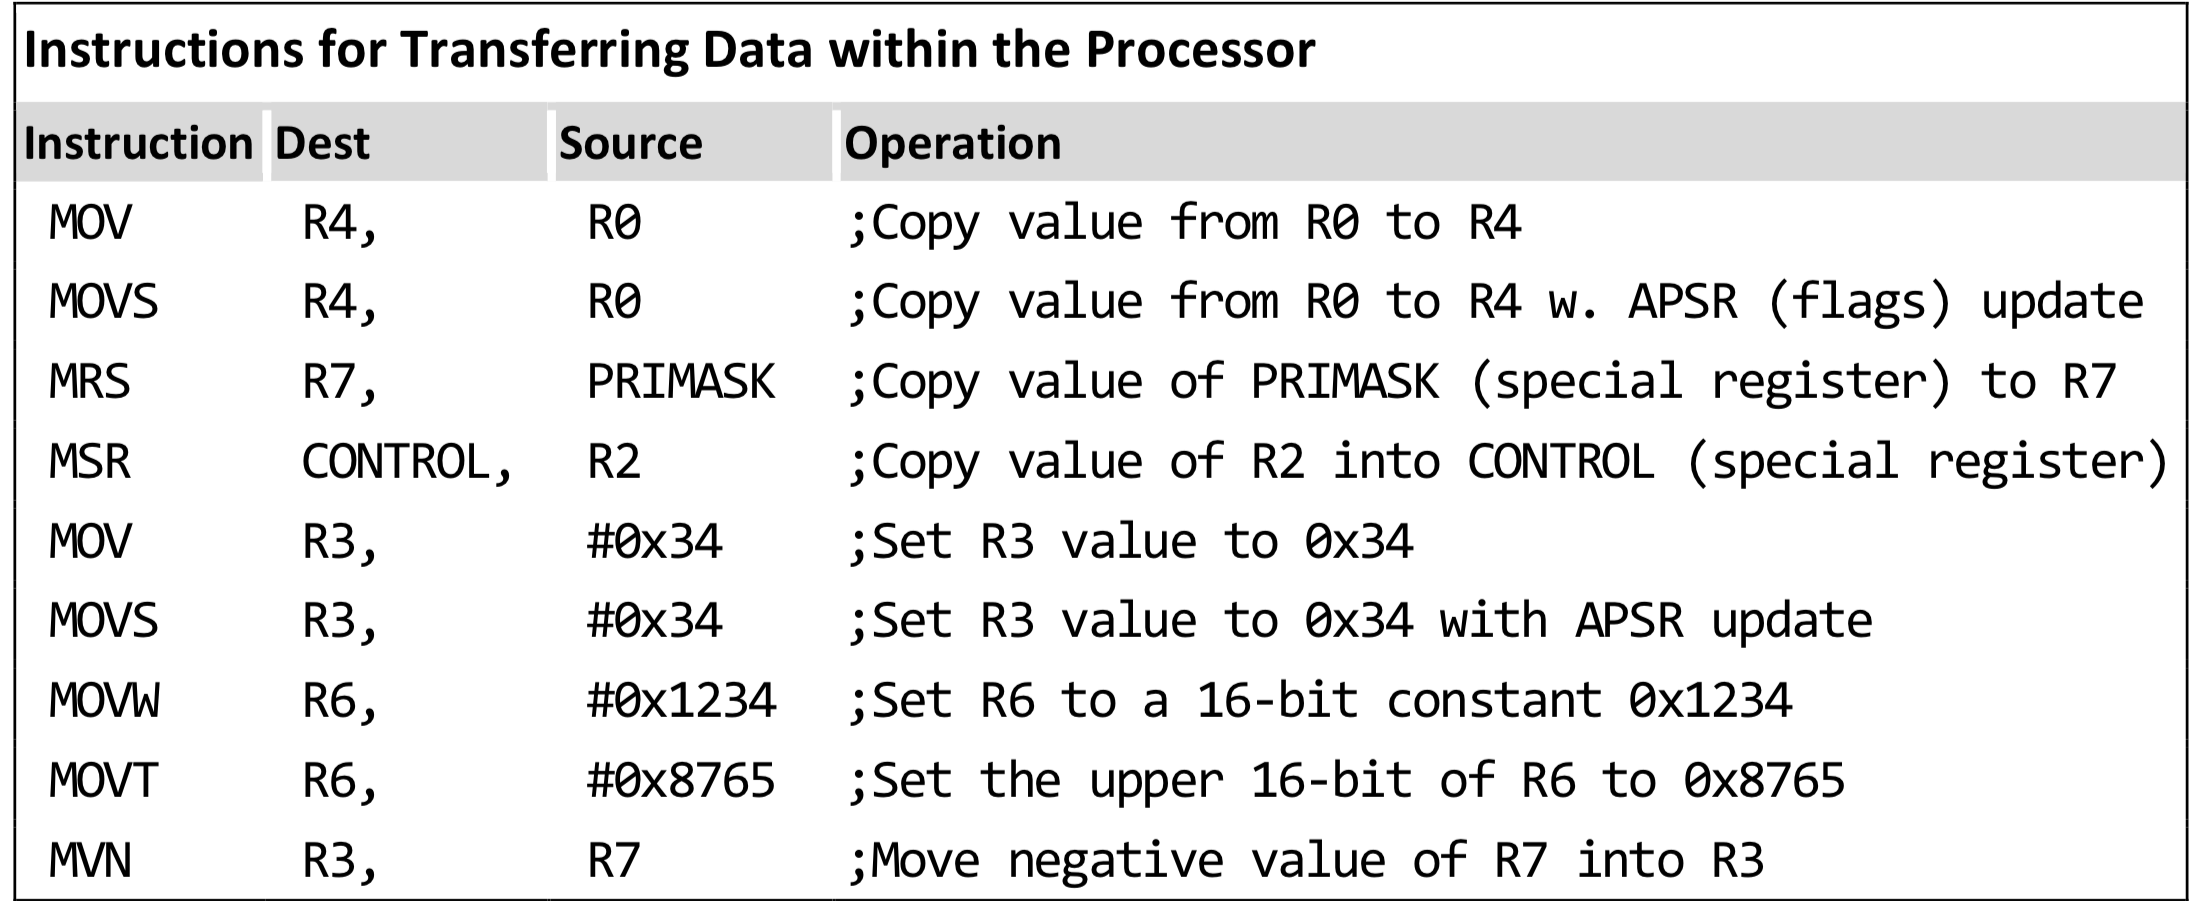
\includegraphics[width=9cm]{images/MOV-Instruktion}
\end{minipage}
%
\begin{minipage}[t]{0.5cm}
	\-\
\end{minipage}
%
\begin{minipage}[t]{9cm}
	\subsection{Memory Access Instructions}
	Der Cortex-M3 verf"ugt "uber viele verschiedene Instruktionen f"ur den Speicherzugriff. Dies wegen den verschiedenen Adressierungsarten und Datengr"ossen. F"ur normale Datentransfers, sind folgenden Instruktionen vorhanden:\\
		
		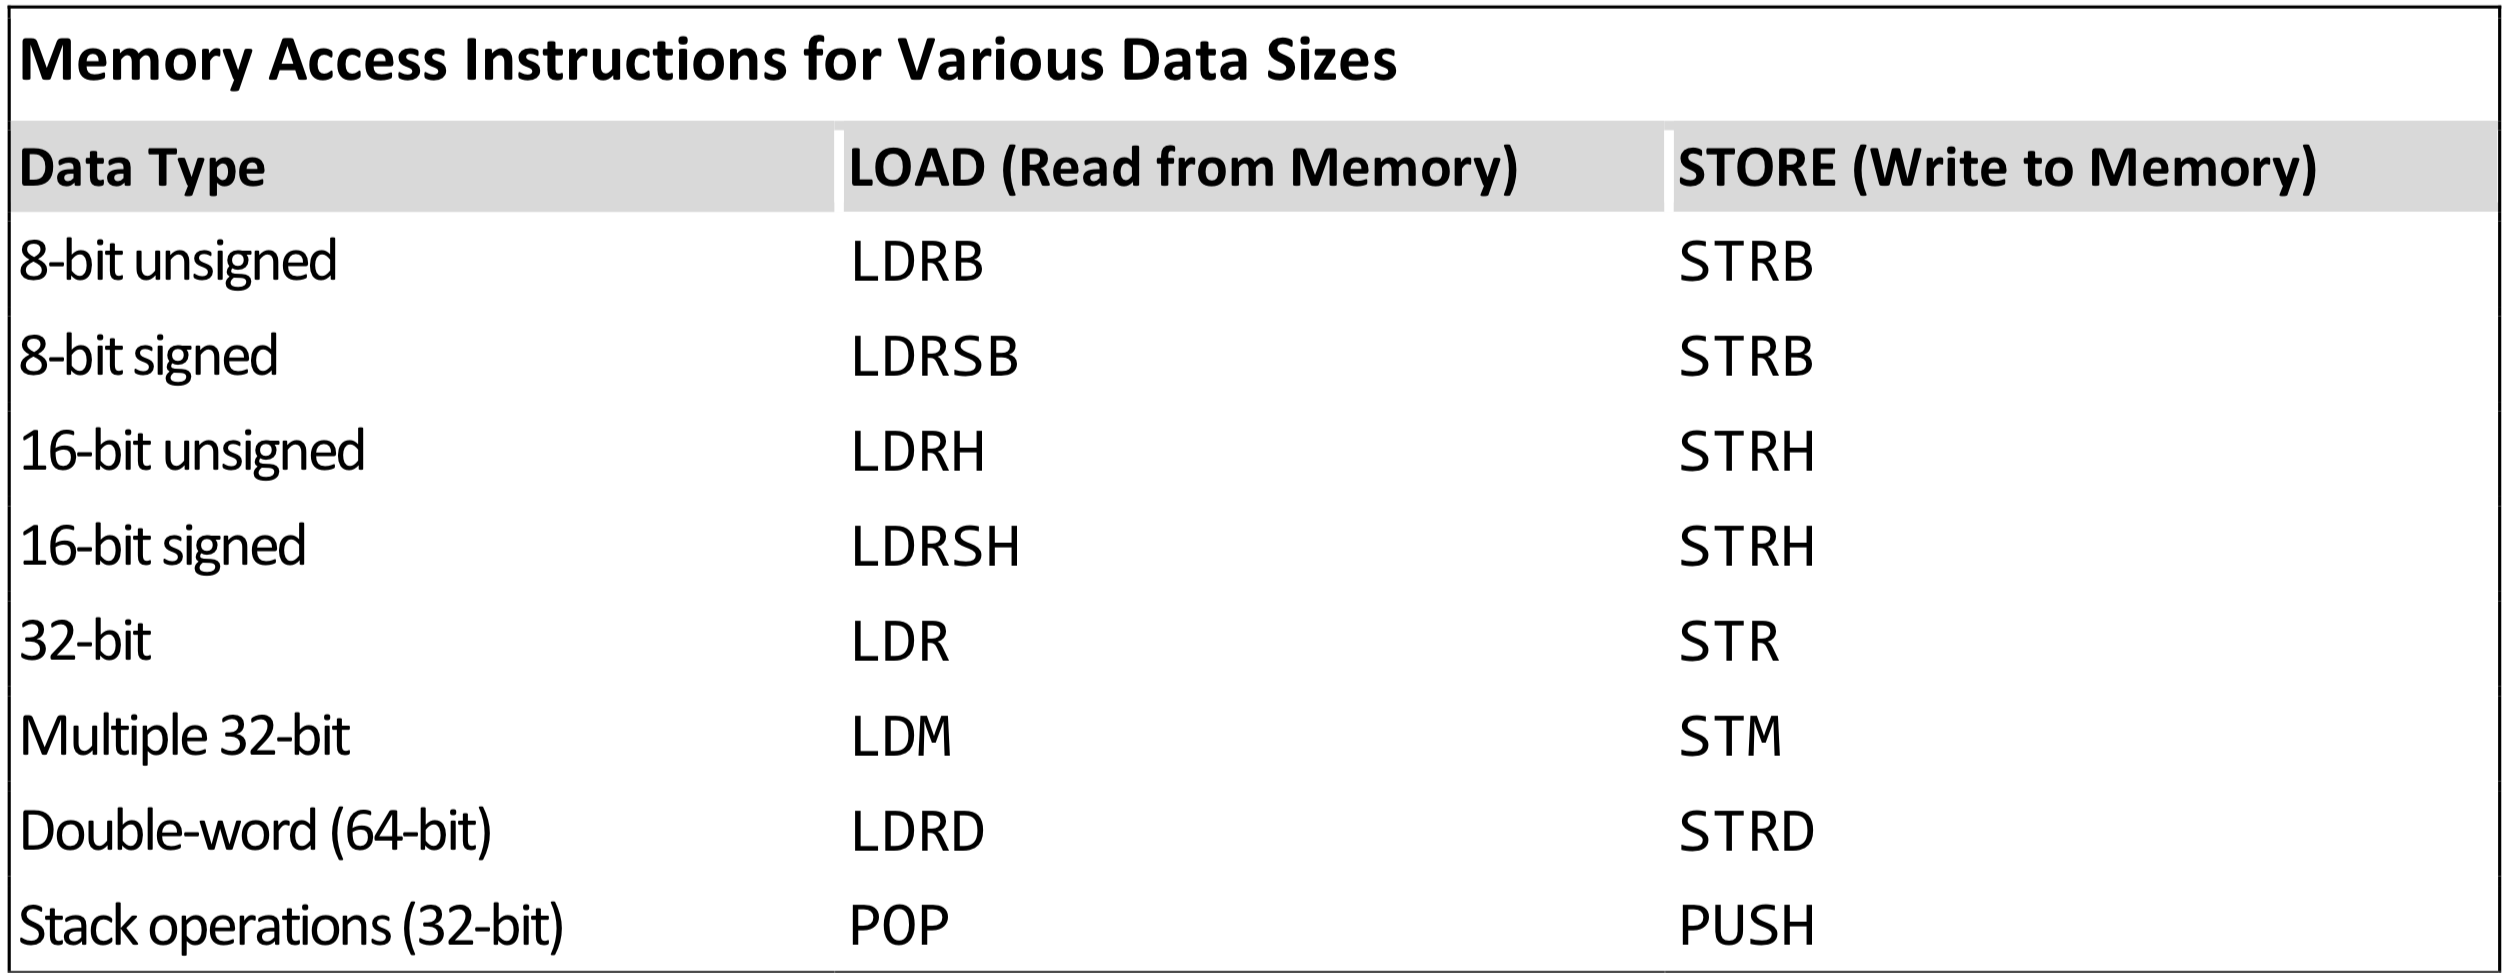
\includegraphics[width=9cm]{images/LDR-Instruktion}
		
		Mit der \textit{LDM} bzw. \textit{STM} Instruktion ist es m"oglich gerde eine ganze Registerliste zu Laden bzw. zu Speichern.
\end{minipage}

\subsection{Stack Push und Pop}
\begin{multicols}{2}
    \begin{minipage}{3cm}
        PUSH \qquad {R0}\newline
        PUSH \qquad {R1}\newline
        PUSH \qquad {R2}\newline
        POP  \qquad {R3}\newline
        POP  \qquad {R4}\newline
        POP  \qquad {R5}\newline
    \end{minipage}
    \begin{minipage}{\linewidth}
        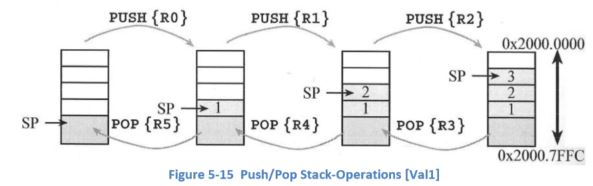
\includegraphics[width=1.5\linewidth]{images/stackpushpop}  
    \end{minipage}
\end{multicols}
 \textbf{\textit{PUSH}} und \textbf{\textit{POP}} k"onnen auch Registerlisten mitgegeben werden, wie folgendes Beispiel zeigt:
 
 \colorbox{lightgray}{
    \begin{tabular}{lll}
        PUSH   & \{R4-R6,LR\}  & ;Save R4 to R6 an LinkRegister at the beginning of a subroutine.\\ 
        && ; LR contains the return address\\
        ...   &   & ;processing the subroutine\\ 
        POP & \{R4-R6,PC\} & ;POP R4 to R6, and return address from stack. The return address\\
        && ;is stored into PC directly, this triggers a branch (subroutine return)
    \end{tabular} }


\subsubsection{Generelle Regeln bei der Verwendung des Stacks}
\begin{minipage}{9cm}
	\begin{enumerate}
        \item Funktionen sollten die gleiche Anzahl Push und Pop Befehle aufweisen.
        \item Stackzugriff nur innerhalb des allozierten Bereichs
        \item Es sollte nicht über den SP auf den Stack geschrieben oder gelesen werden.
        \item Stack sollte zuerst den SP dekrementieren und erst dann die Daten ablegen.
        \item Stack sollte die Daten zuerst lesen und erst dann den SP inkrementieren.
    \end{enumerate}
\end{minipage}
%
\begin{minipage}{0.5cm}
	\-\
\end{minipage}
%
\begin{minipage}{9cm}
	 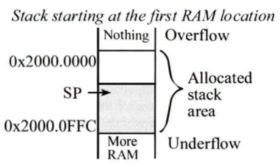
\includegraphics[width=9cm]{images/allocatedStack}  
\end{minipage}

\begin{minipage}[t]{9cm}
	\subsection{Shift and Rotate Instructions}
	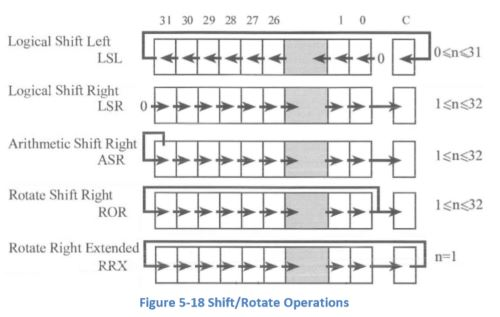
\includegraphics[width=9cm]{images/shiftandrotate}\\
	LSL: Signed, unsigned Multiplikation mit $2^n$\\
	LSR: Unsigned Division mit $2^n$
	
\end{minipage}
%
\begin{minipage}[t]{0.5cm}
	\-\
\end{minipage}
%
\begin{minipage}[t]{9cm}
	\subsection{Bit-Field Processing Instructions}
		Der Cortex-M3/M4 Porzesor verf"ugt "uber viele verschiedene \textit{Bit-Field Processing Operations}-Instruktionen, einzelne sind folgend aufgelistet:\\

		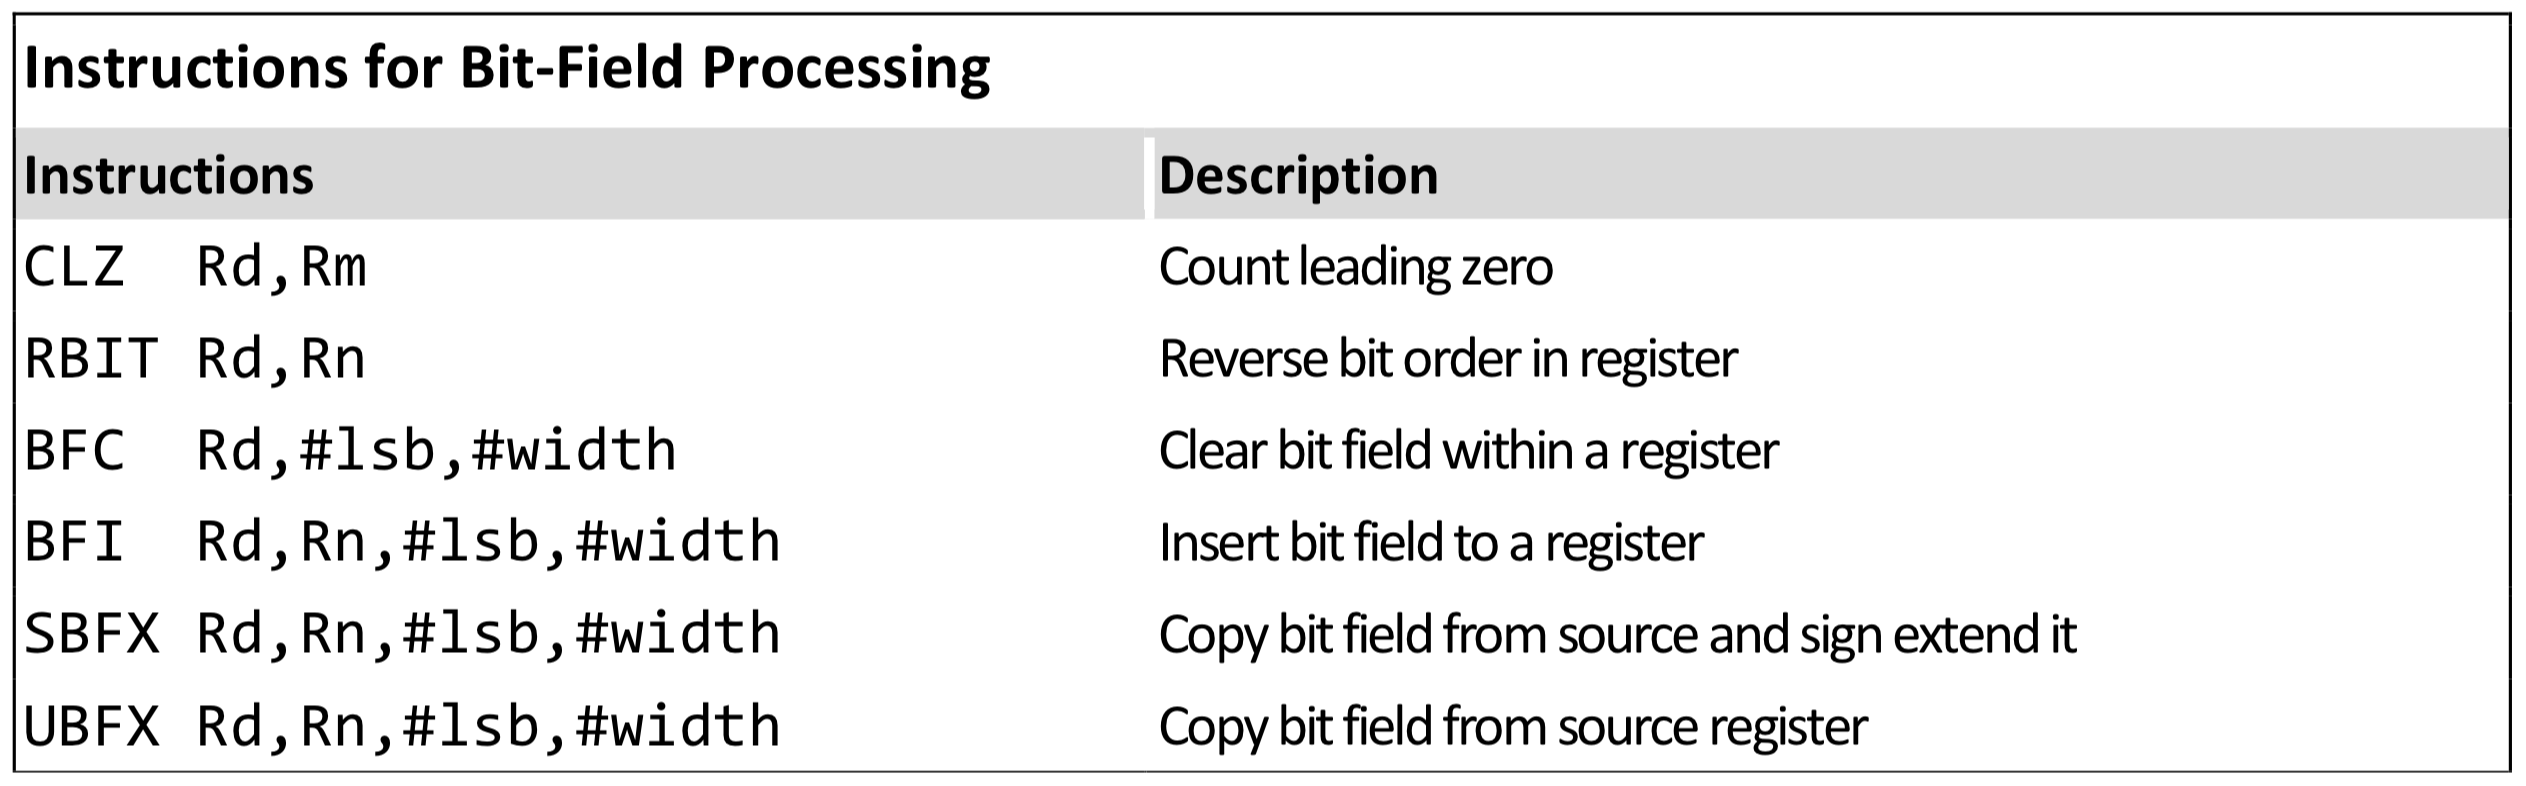
\includegraphics[width=9cm]{images/bit-field-processing}
\end{minipage}


\begin{minipage}[t]{9cm}
	\subsection{Compare and Test}
	Die \textit{\textbf{COMPARE}} und \textit{\textbf{TEST}} Instruktionen aktualisieren die Flags im \textit{APSR}, welche f"ur den \textit{Conditional Branch} oder \textit{Conditional Execution} ben"otigt werden.\\

	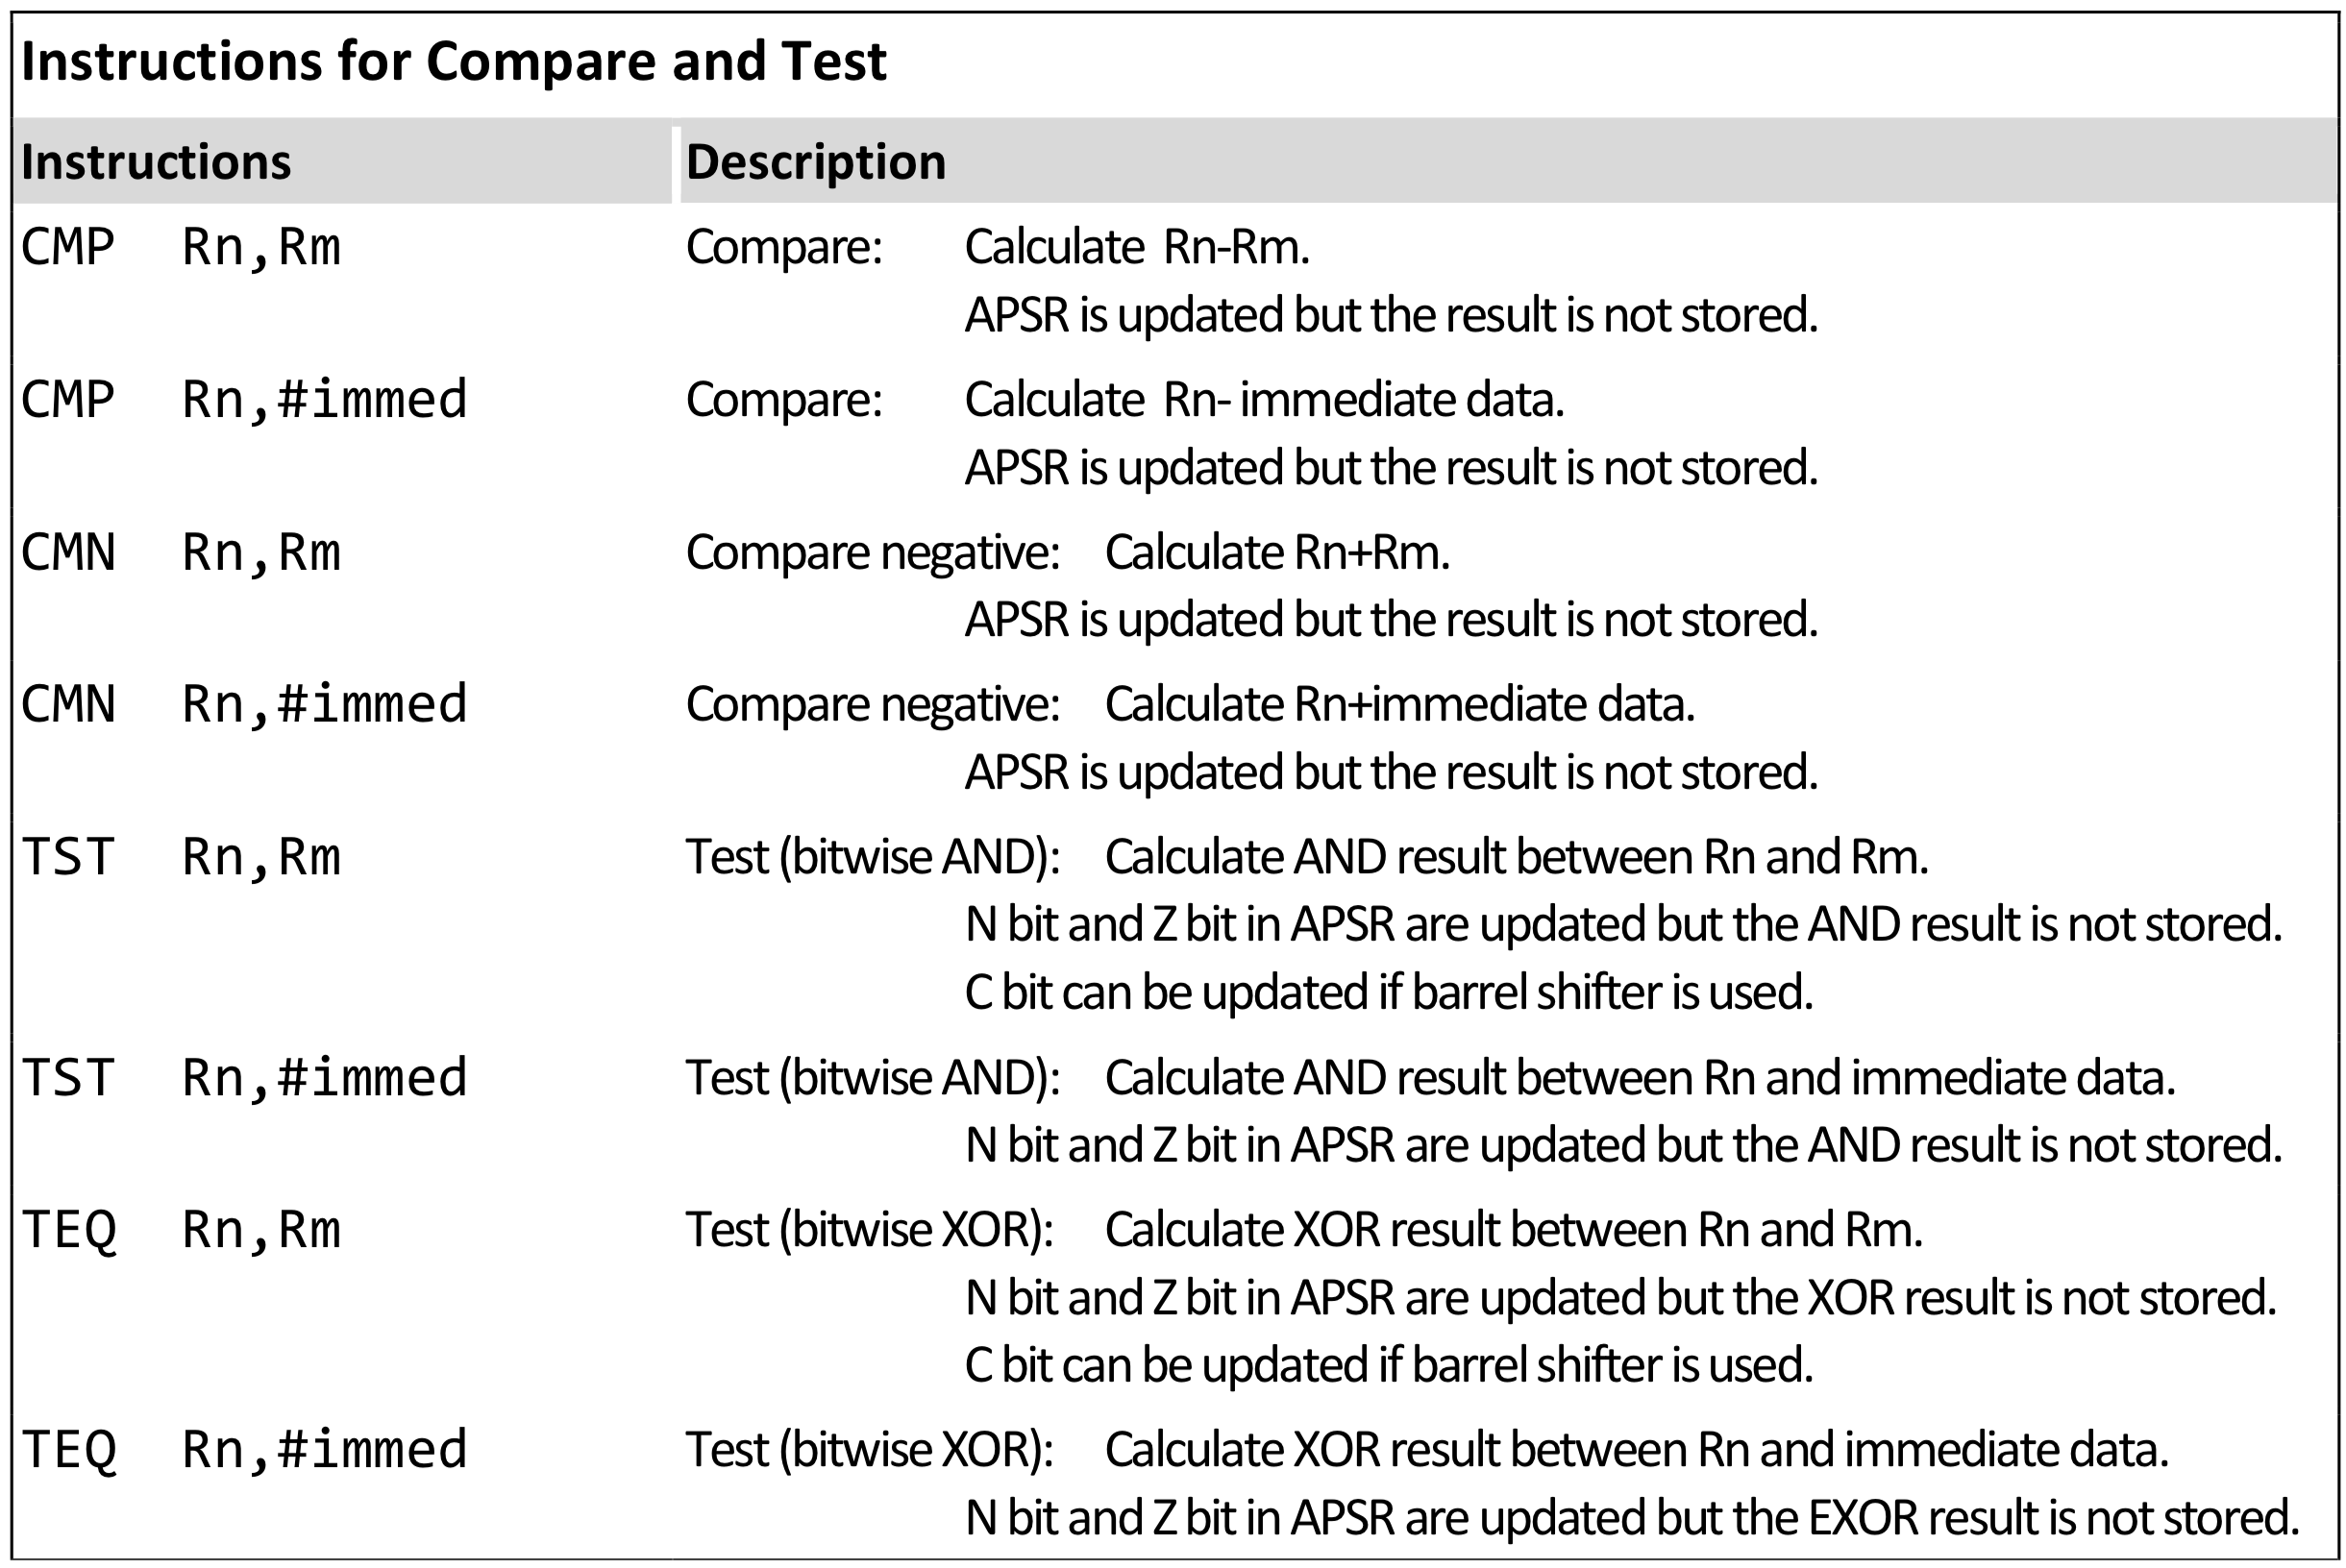
\includegraphics[width=9cm]{images/compare-and-test}

\end{minipage}
%
\begin{minipage}[t]{0.5cm}
	\-\
\end{minipage}
%
\begin{minipage}[t]{9cm}
	\subsection{Program Flow Control}
	\subsubsection{Unconditional Branches}
	\textit{Unconditional Branches} sind Spr"unge zu einem Label, welche wie folgt implementiert werden k"onnen.\\
	
	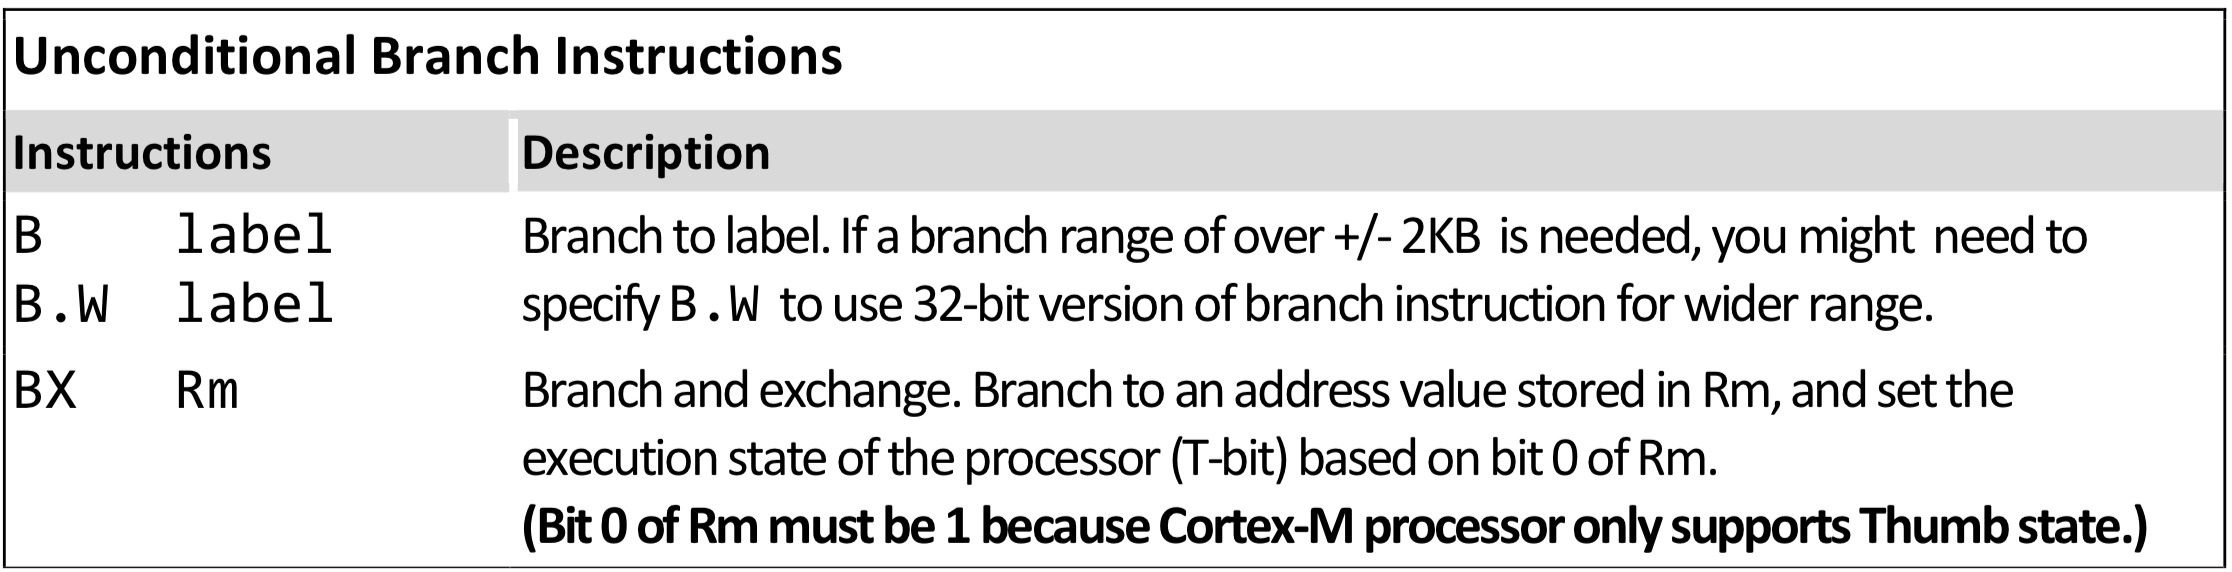
\includegraphics[width=9cm]{images/branches}
	
	\subsubsection{Function Calls}
	F"ur den Funktionsaufruf wird die Instruktion \textit{Branch and Link} verwendet.\\
	
	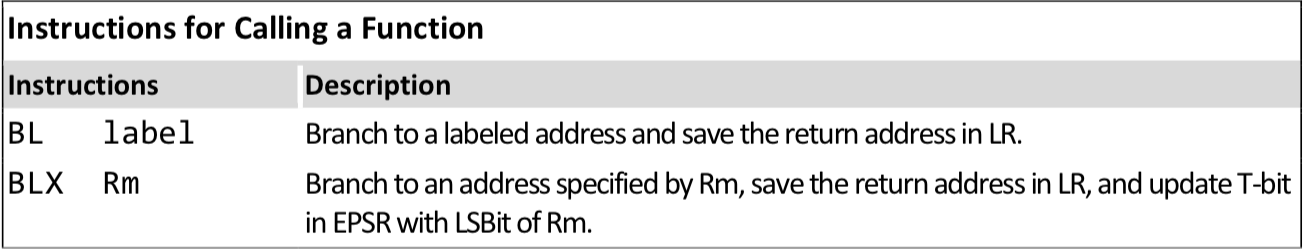
\includegraphics[width=9cm]{images/Function_call}
\end{minipage}


\begin{minipage}{9cm}
	\subsubsection{Conditional Branches}
	\textit{Conditional Branches} sind bedingte Spr"unge, bei welchen nur zur angegeben Adresse gesprungen wird, wenn die Flags die Bedingung erf"ullen. Die Flags (APSR) werden immer vor einem \textit{Conditional Branch} mit einer \textbf{\textit{CMP}}-Instruktion evaluiert.\\
	
	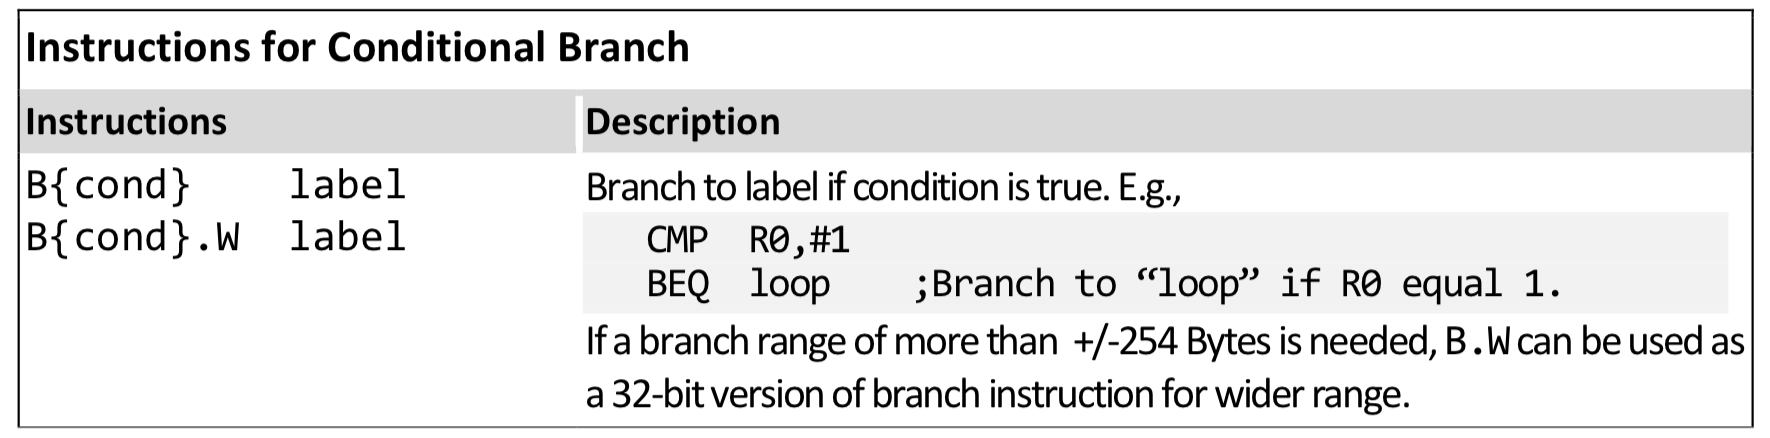
\includegraphics[width=9cm]{images/Conditional_Branch1}
	
	Ein Beispiel:\\
	
	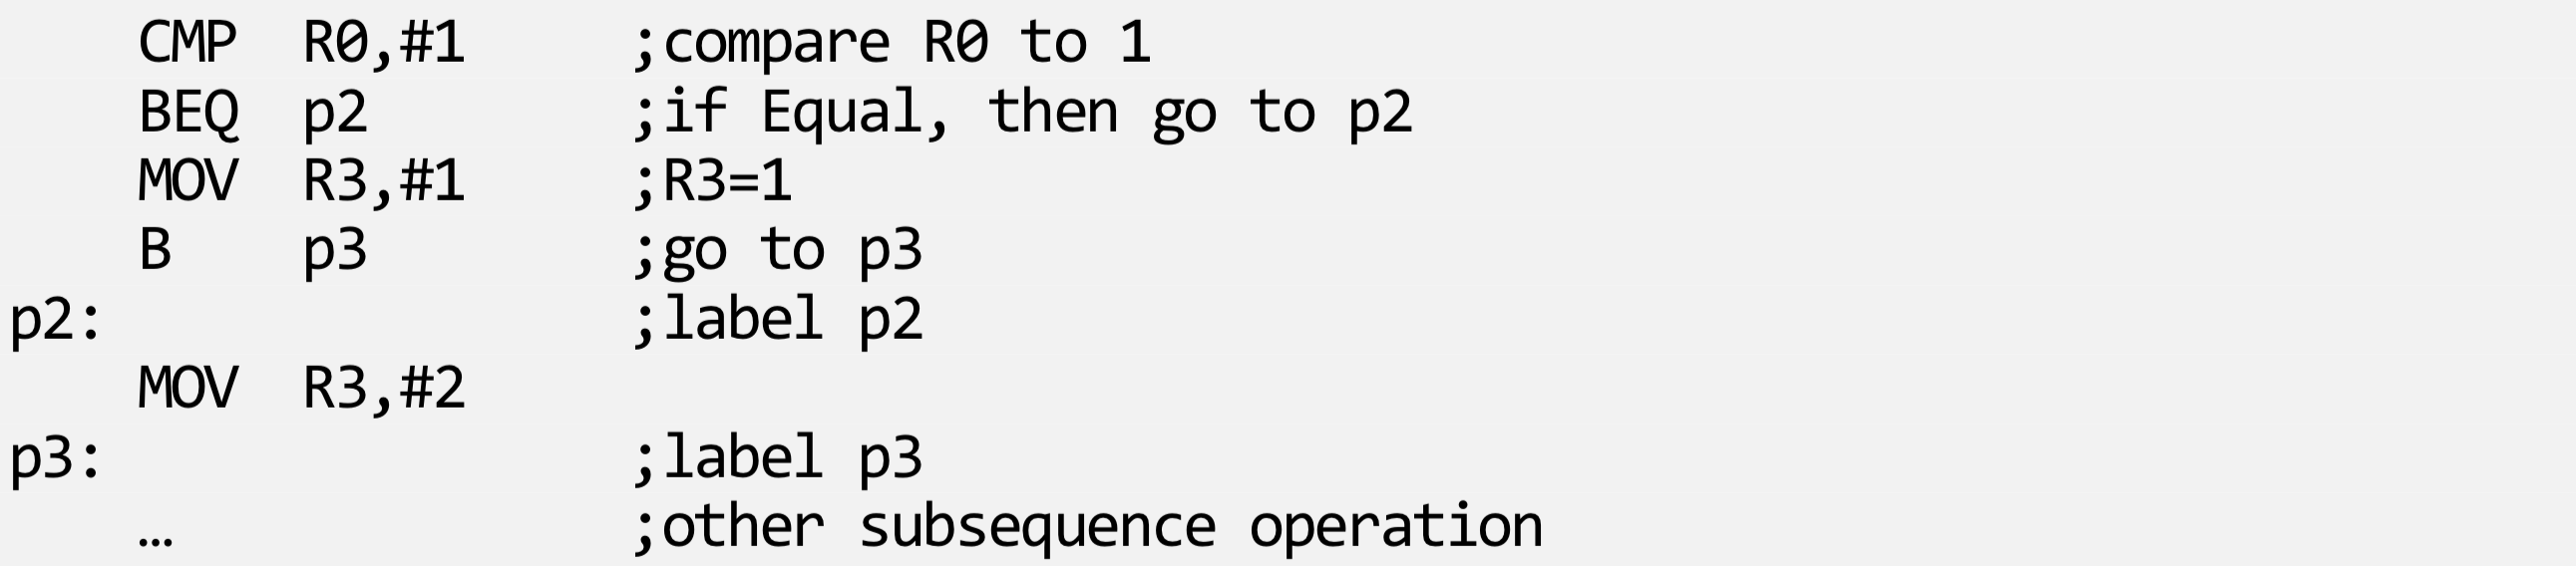
\includegraphics[width=9cm]{images/Conditional_Branch_Bsp}	
\end{minipage}
%
\begin{minipage}{0.5cm}
	\-\
\end{minipage}
%
\begin{minipage}{9cm}
	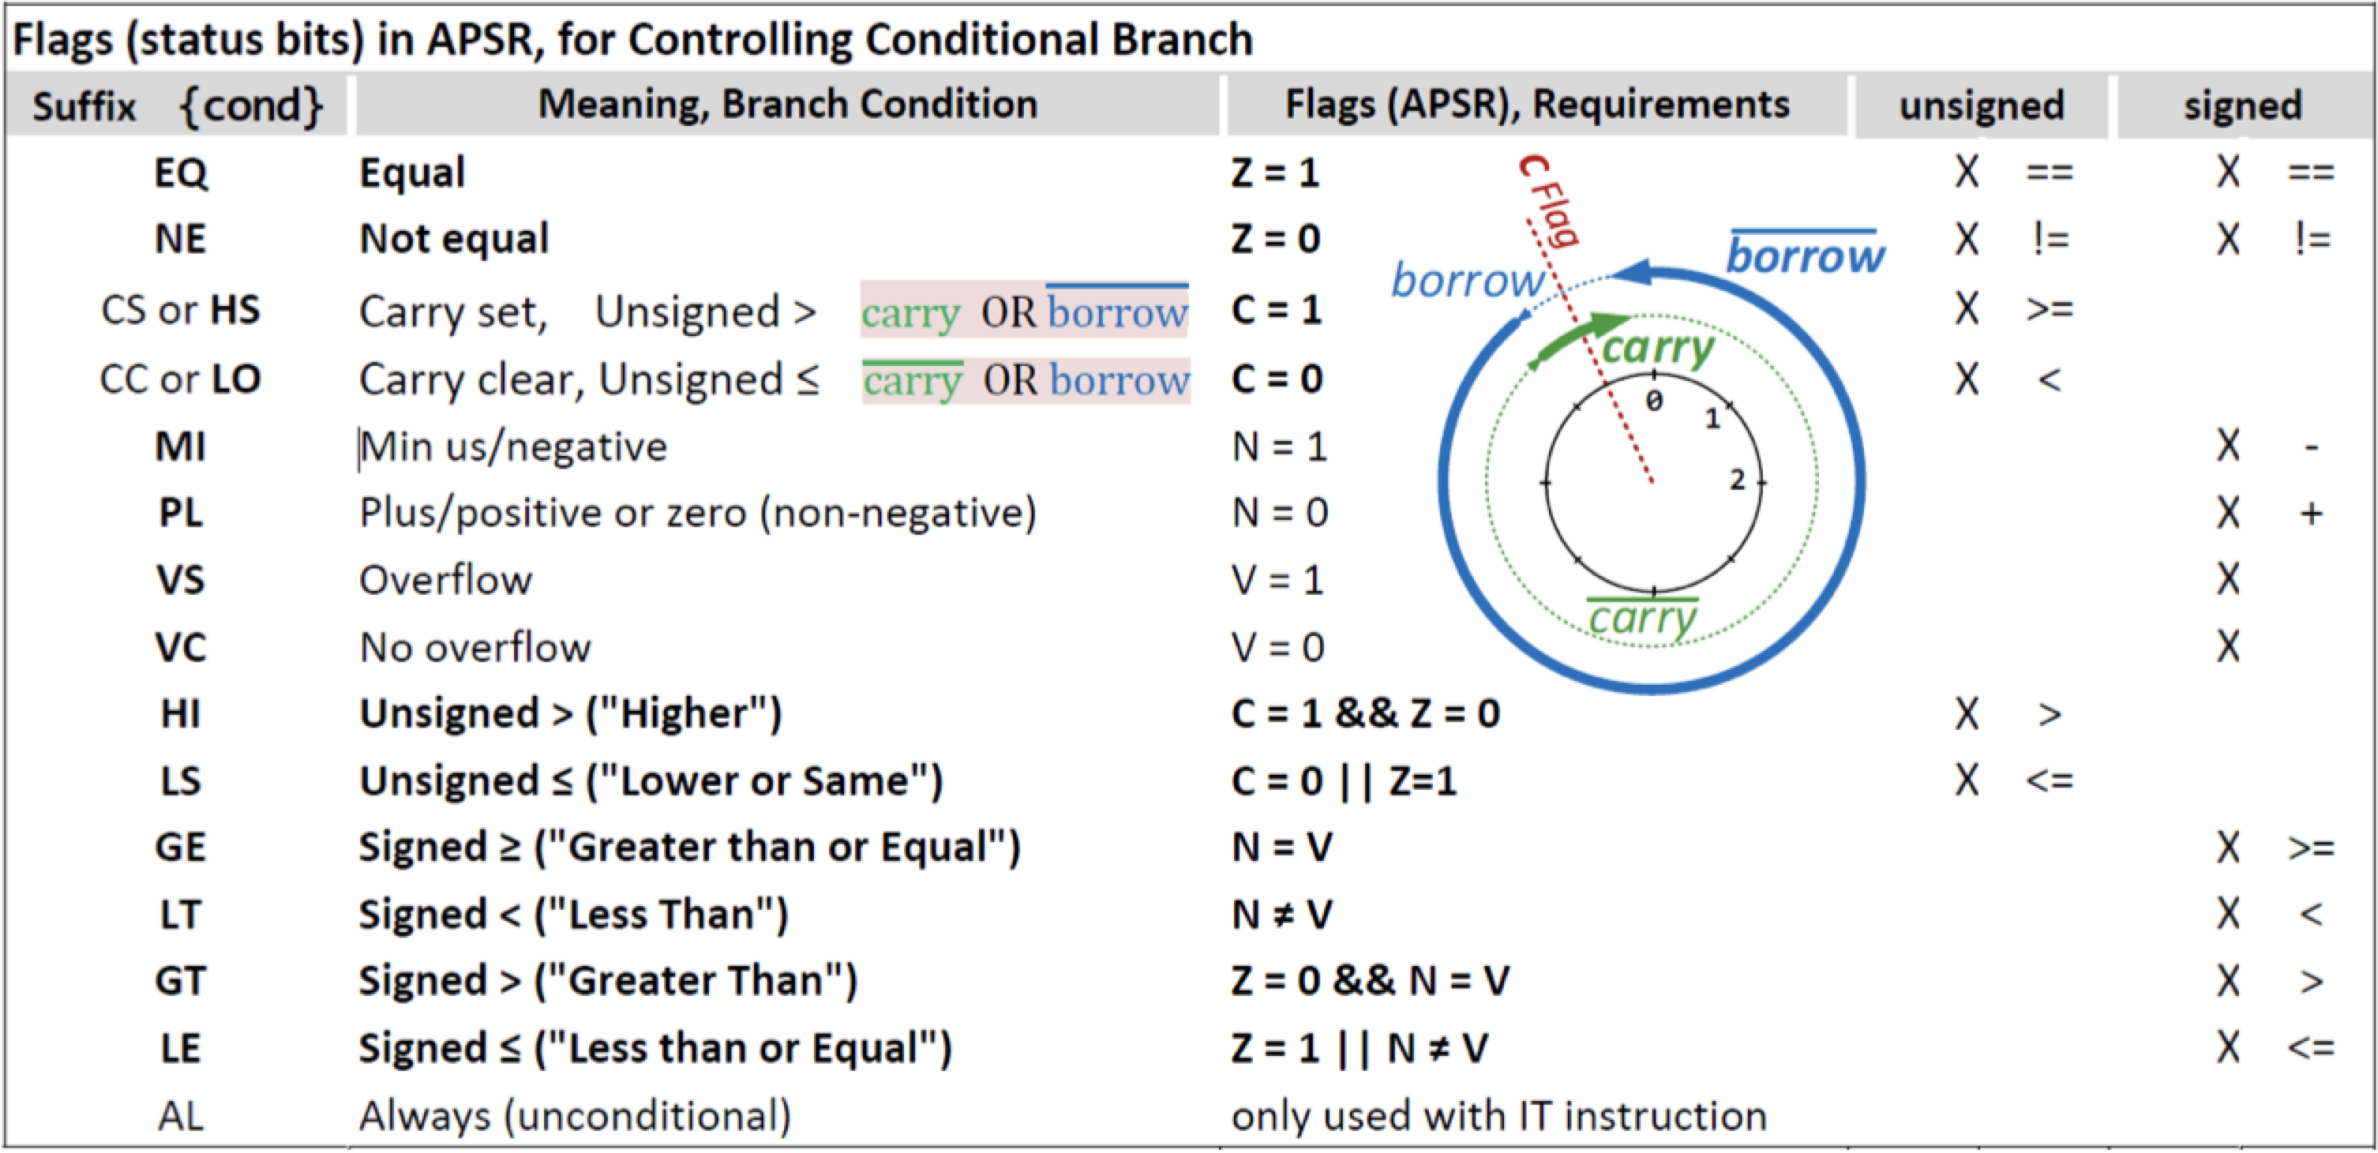
\includegraphics[width=9cm]{images/flags_conditional}
\end{minipage}

	




